\documentclass[9pt,twocolumn,twoside]{pnas-new}
% Use the lineno option to display guide line numbers if required.
% Note that the use of elements such as single-column equations
% may affect the guide line number alignment. 

\templatetype{pnasresearcharticle} % Choose template 
% {pnasresearcharticle} = Template for a two-column research article
% {pnasmathematics} = Template for a one-column mathematics article
% {pnasinvited} = Template for a PNAS invited submission

\usepackage{amsthm}
\usepackage{amsmath}
\usepackage{amssymb}
\usepackage{multicol}


\DeclareMathOperator*{\argmax}{argmax}
\newtheorem{corollary}{Corollary}
\newtheorem{axiom}{Axiom}
\newtheorem{statement}{Statement}
\newtheorem{theorem}{Theorem}
\newtheorem{definition}{Definition}
\newtheorem{lemma}[theorem]{Lemma}

\title{A way around the exploration-exploitation dilemma.}

% Use letters for affiliations, numbers to show equal authorship (if applicable) and to indicate the corresponding author
\author[a,1]{Erik J Peterson}
\author[a,b]{Timothy D Verstynen}
\affil[a]{Department of Psychology}
\affil[b]{Center for the Neural Basis of Cognition, Carnegie Mellon University, Pittsburgh PA}

% Please give the surname of the lead author for the running footer
\leadauthor{Peterson} 

% Please add here a significance statement to explain the relevance of your work
% \significancestatement{We present a deterministic way for an agent to learn how to maximize reward, and to explore their world with both done in an optimal manner. In our approach exploration is done only to maximize information value--a quantity we define axiomatically. Maximizing information value forces the animal to learn a general memory of the world that is not motivated by reward acquisition. An important side effect of this general learning is that reward learning also improves, to optimality. We call this view of the reinforcement learning problem, dual value learning. Dual value learning is a simple way to avoid the exploration-exploitation dilemma. The major cost of our approach is an increase in worst-case sample efficiency.}

% Please include corresponding author, author contribution and author declaration information
% \authorcontributions{EJP?.}
\authordeclaration{The authors have no conflicts of interest to declare.}
% \equalauthors{\textsuperscript{1}A.O.(Author One) and A.T. (Author Two) contributed equally to this work (remove if not applicable).}
\correspondingauthor{\textsuperscript{1}To whom correspondence should be addressed. E-mail: Erik.Exists@gmail.com}

% Keywords are not mandatory, but authors are strongly encouraged to provide them. If provided, please include two to five keywords, separated by the pipe symbol, e.g:
% \keywords{Keyword 1 $|$ Keyword 2 $|$ Keyword 3 $|$ ...} 

% Short abstract
\begin{abstract}
The exploration-exploitation dilemma is a fundamental but intractable problem in the learning and decision sciences. 
% TODO example: explain the common view
Here we challenge the common view of the dilemma--which focuses only on reward--by breaking into a tractable two-part problem, creating separate mathematical objectives for exploration and exploitation. To value exploration independently of reward, we develop a new set of values axioms inspired by Shannon's original approach to developing information theory. We then turn to field of computer science, and the method of dynamic programming, to develop a provably optimal (greedy) algorithms that maximize both information value and reward. The cost of this solution is an increase in worst-case sample efficiency when compared to a equivalent reinforcement learning problem. The severity of the cost depends on the size of the environment and the rate of rewards.
\end{abstract}

% \dates{This manuscript was compiled on \today}
% \doi{\url{www.pnas.org/cgi/doi/10.1073/pnas.XXXXXXXXXX}}

\begin{document}
\verticaladjustment{-2pt}
\maketitle

% TODO: talk about how max E can reduce bias in ML algs, as discussed by: 
% Perspective | Published: 09 April 2019
% Lessons for artificial intelligence from the study of natural stupidity
% https://www.nature.com/articles/s42256-019-0038-z
% the r + bI approach can not reduce bias in the same way?

\thispagestyle{firststyle}
\ifthenelse{\boolean{shortarticle}}{\ifthenelse{\boolean{singlecolumn}}{\abscontentformatted}{\abscontent}}{}
When placed in a new environment a rat will explore it even if no tangible rewards, like food and water, are expected \cite{Liu2019,Jaegle,Todd2015}. Sometimes they'll explore even when it is certain that exploration will lead to a loss \cite{ZheWang2019}. If a reward is expected though, an animal will generally explore and discover it \cite{Todd2015}. This exploration gets interpreted as the animal exploring \textit{for} reward--to maximize reward \cite{Sutton2018}. Here we offer an alternative view: animals don't explore to maximize reward at all, they explore to maximize information--sometimes--about reward. 

% Schmidhuber layed out the theoretical groundwork for our view of exploration. He conjectured that \textit{information about the world is valuable for its own sake} \cite{Schmidhuber1991} and argued that, \textit{in addition} to searching for rewards, animals seek to explore to build a model of the world. In doing this he said they are motivated by information itself, as a curiosity signal. In developing this theory, Schmidhuber made the seemingly parsimonious choice that when it comes time optimize, information and reward terms be combined into a single objective function (similar to our Eq.\ref{eq:total_r_I}). This mathematical form set the stage for decades of productive work on rewards, fictive rewards, and curiosity learning \cite{Pathak2017,Sutton1990,dayan1996exploration}. Despite the success including information and reward as a single additive objective suffers from at least one drawback: exploration itself becomes an intractable mathematical problem, fundamentally limited by the partial observability of rewards \cite{thrun1992active,dayan1996exploration,findling2018computational,gershman2018deconstructing} 

% Here we make a stronger conjecture than Schmidhuber's \cite{Schmidhuber1991}. We assert that information is valuable \textit{entirely} for its own sake. This lets us completely separate reward and information into two objectives, whose values we independently maximize. Estimating dual values is less simple than having a single objective, but the increase in complexity comes with a theoretical benefit. Exploration becomes a tractable mathematical problem, one we can solve deterministically.

Our contribution is threefold. We first set out a series of axioms to serve as principled basis for information value, and use these to implement a working scheme rooted in information theory. Next we develop an optimal policy for exploration that maximizes information value. This theory is purely deterministic, so exploration no longer relies on random sampling \cite{Haarnojaa,Kakade2002,Pathak2017,Sutton1990,thrun1992active,dayan1996exploration}. Finally we derive a new myopic controller \cite{Hocker2017}, a \textit{meta-policy}, that allows for simultaneously optimal and deterministic solutions to both problems of exploration and exploitation. 

% TODO needs work; goes where?
% The intuition for how our more complex dual approach can be optimal, when the simpler additive approach can't be, rests on when the trade-off to explore or exploit is made. When working with a single additive objective one must find an optimal way to balance curiosity and reward \textit{at every time-point, at the same time}. By separating terms, one only has to balance \textit{when to pursue each objective}; It becomes a problem of time-sharing. Time sharing can be a much simpler and more tractable problem.


Exploration is almost universally regarded as stochastic process \cite{Sutton2018,Jaegle}. Before moving to stochastic view, we considered a deterministic approach. We'll show how to recast exploration as a deterministic search process. Specifically, we'll borrow a tool from computer science and cast exploration as a dynamic programming problem \cite{TODO}. To do this we need to make an additional assumption about animal learning.

% --------------------------------------------------------------------------
\subsubsection*{A Bellman solution}
If $M$ has optimal substructure, we can use the Bellman equation \cite{Bellman} to write down an optimal (greedy) policy for maximizing information value $E$ over the time horizon $T$ is given by Eq.~\ref{eq:V_star}.

\begin{equation} \label{eq:V_star}
    \begin{split}
        V^*_{\pi_E}(M_0) = \max_{a \in A} \sum_{t \in T} F(M_t, a_t)
    \end{split}
\end{equation}

By theorem~\ref{theorem:opt_sub}, memory $M$ has optimal substructure which means Eq.~\ref{eq:V_star} can be decomposed into a series of local greedy decisions.

\begin{equation} \label{eq:bellman_seq}
    \begin{split}
        V^*_{\pi_E}(M_0) &= \max_{a \in A} \Big [\sum_{t \in T} F(M_t, a_t)\Big ]\\
                         &= \max_{a \in A} \Big [F(M_0, a_0) + \sum_{t \in T} F(M_{t+1}, a_{t+1})\Big ]\\
                         &= F(M_0, a_0) + \max_{a \in A} \Big [\sum_{t \in T} F(M_{t+1}, a_{t+1}) \Big ]\\
                         &= F(M_0, a_0) + V^*_{\pi_E}(M_{t+1}) + V^*_{\pi_E}(M_{t+2}),\ \ldots
    \end{split}
\end{equation}

From the final entry in Eq.~\ref{eq:bellman_seq}, we can write down an optimal recursive value function for the current memory $M_0$ in terms of the next memory $M_1$ (Eq.~\ref{eq:bellman_iter}).

\begin{equation} \label{eq:bellman_iter}
    V^*_{\pi_E}(M_{t}) = F(M_{t}, a_{t}) + \max_{a \in A} \Big [ [F(M_{t+1}, a_t) \Big ]
\end{equation}
    
Theorem~\ref{theorem:opt_sub} and Eq~\ref{eq:bellman_seq} demonstrate how to optimally maximize information value, given an optimal initial payoff $F(M_0, a_0)$. The question then is how find this first value optimally; A key step needed for all optimal dynamic programming solutions. To do this we imagine we have a vector of $K$ possible payoffs $F_0 \in \mathbb{R}^K$, which is the same size as our action space $A$. If all the values of $F_0$ are equal, then under a greedy policy any choice is a good as any other--so any choice is optimal. We restrict the initial value to $F_0 > 0$.  % TODO explain why, gently.

% ---------------------------------------------------------------------------
\subsection*{Exploration as a dynamic programming problem}
The dynamic programming solution to maximize information value is also a dynamic programming solution for exploration. By making a weak assumption on the learning of $M$, we can prove that our greedy policy $\pi^*_E$ leads to a complete and exhaustive exploration of any finite space $S$. Specifically, we show:

\begin{enumerate}[noitemsep,wide=0pt,leftmargin=\dimexpr\labelwidth+2\labelsep\relax]
    \item The optimal policy $\pi^*_E$ must visit each state in $s \in S$ at least once.
    \item The optimal policy $\pi^*_E$ must revisit each $s \in S$ until learning about each state $s$ plateaus when $g(M_{t+1}, s) = g(M_{t},s)$.
\end{enumerate}


% HERE: re-write this assumption using f. Weaken it compared to below. Convex doesn't matter.
\subsection*{Exploration during reinforcement learning}
The overall objective in reinforcement learning is to maximize $V_{\pi_R}$, the expected value of total future rewards (Eq~\ref{eq:total_r_I}) \cite{Sutton2018}. Here we use the term $I_t$ as a generic stand in for a range of fictive rewards, including novelty bonuses \cite{Kakade2002}, curiosity signals \cite{Pathak2017}, Bayesian updates \cite{Radulescu2019}, or entropy terms \cite{Haarnoja2015,Haarnoja2017}.  Often the fictive term in these equations is arbitrarily re-weighted. We use $\beta$ for this fictive weight. Likewise, rewards are denoted by $R_t$. In this example the total time $T$ is said to be finite, simplifying the notation.

\begin{equation}
    V_{\pi_R} = \sum_{t \in T, s \in S} R_t + \beta I_t
    \label{eq:total_r_I}
\end{equation}

Explicitly, we propose that reinforcement learning problems should try and optimize two values: reward (Eq.~\ref{eq:total_r_2}) and information (Eq.~\ref{eq:total_e}). 

\begin{multicols}{2}
  \begin{equation}
    V_{\pi_R} = \sum_{t \in T, s \in S} R_t
    \label{eq:total_r_2}
  \end{equation} \break
  \begin{equation}
    V_{\pi_I} = \sum_{t \in T, s \in S} I_t
    \label{eq:total_e}
  \end{equation}
\end{multicols}

We separate the objectives because classical rewards and information value have fundamentally different philosophical and mathematical properties. Conflating them introduces an undesirable bias, both in trying to maximize information value and in maximizing rewards.

\subsection*{Biased by reward}
Exploration often means a loss of rewards. To motivate exploration, lost rewards are often re-balanced with information gains, novelty signals, or other fictive reward signals. This is simple and intuitive, but comes with an under-appreciated limitation. If the true goal is to maximize total reward $R$, adding a fictive reward obscures this aim. After all, now an increase in $V_{\pi_R}$ may come from $R$ or from the fictive term $\beta I$. So while fictive rewards do encourage exploration they offer no guarantee of a performance increase in $R$, or in the long-term value $V_{\pi_R}$. 

Conversely, if an animal wants to build a generally useful model of world, as Schmidhuber suggests, then biasing choices by maximizing reward is suboptimal. Both in terms of maximizing both the accuracy of the world model (which will wind up over-sampled near rewarding sites), and the efficiency with which the model is built (much time is wasted gathering rewards). 

% ----------------------------------------------------------------------------
\subsection*{Information is not a reward}
Information and reward so seem to have opposing properties. If a rat shares a potato chip with a cage-mate, it must break the chip up to share, leaving has less food for itself. While if a student shares an idea with a lab-mate, the is idea is not divided up or lost. Thus rewards are a conserved resource, information is not. 

The same kind of reward can be consumed many times without necessarily losing value\footnote{In practice, there are satiety effects but these are not a necessary part of the reward's value}. Information once learned though has no value in being be learned again. Eating one potato chip often means wanting another, whereas if you know the capital of the United States, there is no value in being told the capital of the United States is Washington DC.

These two philosophical differences suggest that reward and information may also have notable mathematical differences. To evenly share a reward $r$ between $n$ others, $r_n = \frac{r}{n}$. In contrast, information value can, in principle, be shared without loss, i.e., $I_n = I$. Likewise, if an animal is learning about some state of world $s$ the value of information about $s$ should decrease with time. Assuming learning can asymptote, then as $t \rightarrow \infty, I_s \rightarrow 0$. For rewards, value never changes. So as $t \rightarrow \infty, r_s \rightarrow r_s$.\footnote{Though including reward satiety effects may somewhat diminish $r_s$ in practice.} In summary, information is fundamentally not a reward. Information about the world and the rewards from the world are very different kinds of things.

% ---------------------------------------------------------------------------
\subsection*{A way around the dilemma}
We introduce now a new style of reinforcement learning we call \textit{dual value learning}. We conjecture that from point of the view of an animal learning to explore its world \textit{and} gather the most rewards, it can, and probably should, use two different policies for each aim. 

Having two policies $\pi_E$ and $\pi_R$ sidesteps the exploration-exploitation dilemma in the following ways. Exploration now generates tangible value, and so is not in any sense costly. Because of this exploration can be carried out completely. In turn this ensures the reward policy $\pi^*_R$ discovers its global optimum, if it exists. In circumstances where the environment can be learned $E$ will decay to $\epsilon \geq 0$ leaving $\pi^*_R$ in control, and so exploitation becomes the final policy. When the environment changes exploration can begin again, as $\pi^*_E$ resumes intermittent control. Finally, while only one policy can control behavior each policy can learn from the actions of the other. This makes learning to maximize exploration and exploit rewards cooperative, even though action control is competitive. 

One policy can drive behavior at a time. To adjudicate, we derive a simple, value-based, myopic controller \cite{Hocker2017} to select which policy dominates. We call this policy on policies a \textit{meta-policy} and denote it by $\pi_{\pi}$. We insist that for any meta-policy to be considered valid meta-policy it must inherit any optimality present in $\pi^*_E$ \textit{and} $\pi^*_R$.

We base our formulation for $\pi_{\pi}$ in Eq~\ref{eq:meta_greedy} on the asymptotic properties of information and rewards. To review, $E_t \rightarrow \epsilon$ as $t \rightarrow T$ (Theorem~\ref{theorem:Z}) which implies that as $T \rightarrow \infty$ then $V_{pi_E} \rightarrow \epsilon$. Reward, on the other hand does not decay with time and so $V_{pi_R}$ can grow without bound. A cartoon example of this is depicted in Figure~\ref{fig:simple_E_R_timecourse}.

\begin{equation} \label{eq:meta_greedy}
    \begin{split}
        \pi_{\pi} = 
        \begin{cases}
            \pi_E & : E_t - \epsilon > R_t \\
            \pi_R & : R_t \geq E_t - \epsilon \\
        \end{cases}\\
        \text{subject to the constraints}\\
        R_t \in \{0, 1\}\\ 
        p(R_t = 1) < 1\\
        E_t - \epsilon > 0
    \end{split}
\end{equation}

\begin{figure}
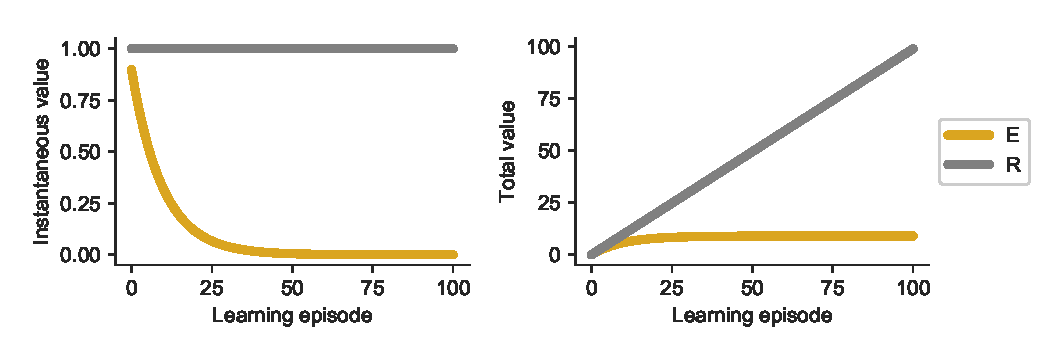
\includegraphics[width=0.5\textwidth]{figures/simple_E_R_timecourse.eps}
\caption{
    \textit{Simulated learning of information and reward value, assuming a linear reward accrual and an exponential decay information value. 
    \textbf{a.} Instantaneous value over 100 learning epochs.  
    \textbf{b.} Average value over 100 learning epochs.}
}
\label{fig:simple_E_R_timecourse}
\end{figure}

Note that to satisfy $E_t - \epsilon > 0$ in Eq~\ref{eq:meta_greedy}, $\epsilon = 0$ when $\Lambda(.)$ is deterministic. Only when the environment is stochastic can $\epsilon$ safely exceed 0.

The meta-policy $\pi_{\pi}$ is a myopic in the sense that at every time $t$, $\pi_E$ or $\pi_R$ has the opportunity to take control but this control lasts only a single time step. There are many other possible meta-policies which could also inherit the optimality of our dual policies. We chose this form for its simplicity, but justify it as similar myopic controls have proven effective for other complex, high variance, problems in neuroscience \cite{Hocker2019}.

Even though the individual policies in the meta-policy are independent, learning can be done in parallel. Regardless of which policy is in control, they can in principle observe choices made by the other and learn from them.   

\begin{theorem}[Optimality of $\pi_{\pi}$] \label{theorem:meta}
    Assuming an infinite time horizon, if $\pi_E$ is optimal and $\pi_R$ is optimal, then $\pi_{\pi}$ is also optimal in the same sense as $\pi_E$ and $\pi_R$.
\end{theorem}
\begin{proof}
    The optimality of $|\pi_{\pi}$ can be seen by direct inspection. If, $p(R = 1) < 1$ and we have an infinite horizon, the $\pi_E$ will have a unbounded number of trials meaning the optimally of $P^*$ holds. Likewise, $\sum E < \epsilon$ as $T \rightarrow \infty$, ensuring $pi_R$ will dominate $\pi_{\pi}$ therefore $\pi_R$ will asymptotically converge to optimal behavior.
\end{proof}

In proving the total optimality of $\pi_{\pi}$ we limit the probability of a positive reward to less than one, denoted by $p(R_t = 1) < 1$. Without this constraint the reward policy $\pi_R$ would always dominate $\pi_{\pi}$ when rewards are certain. While this might be useful in some circumstances, from the point of view $\pi_E$ it is extremely suboptimal as the model would never explore. Limiting $p(R_t = 1) < 1$ is reasonable constraint, as rewards in the real world are rarely certain. A more naturalistic but complex way to handle this edge case would be to introduce reward satiety, and have reward value decay asymptotically with repeated exposure. 


\subsubsection*{An optimally rewarding policy}
If learning during $\pi_{\pi}$ is allowed to continue until $\pi_E$ converges so $E_t - \epsilon = 0$ then, by definition the animal will have completely explored its world. This implies that in turn $\pi_R$ has seen every state, and so can then choose the overall optimal value. Thus is there is a globally optimally reward policy, $\pi_{\pi}$ guarantees it will be found. Classic reinforcement learning views this search as costing potential reward. Dual value learning instead asserts a net gain. Either from information value, from rewards, or both. We suggest that rather than being fundamental, the exploration-exploitation dilemma follows from asking too little from an animal's learning objectives.

% ---------------------------------------------------------------------------
\subsection*{E is satisfied by KL}
The Kullback--Leibler divergence (KL) is a widely used information theory metric, which measures the information gained by replacing one distribution with another. It is highly versatile and widely used in machine learning \cite{Goodfellow-et-al-2016}, Bayesian reasoning \cite{Itti2009,Friston2016}, visual neuroscience \cite{Itti2009}, experimental design \cite{Lopez-Fidalgo2007}, compression \cite{Mackay,Still2012} and information geometry \cite{Ay2015}, to name a few examples. Using a Bayesian approach, Itti and Baladi \citep{Itti2009} developed an approach similar to ours for visual attention, where our information value is identical to their \textit{Bayesian surprise}. Itti and Baladi (2009) showed that compared to range of other theoretical alternative, information value most strongly correlates with eye movements made when humans look at natural images. Again in a Bayesian context, KL plays a key role in guiding \textit{active inference}, a mode of theory where the dogmatic central aim of neural systems is make decisions which minimize (probabilistic) free energy \cite{Friston2016,Schwartenbeck2019}. 

The Kullback--Leibler ($KL$) divergence satisfies all five value axioms (Eq.~\ref{eq:KL}). In expressing $E$ in terms of KL it also allows us to more concretely demonstrate the mathematical properties implied in our axioms.
 
\begin{equation}
    KL(M', M) = \sum_{s \in S} M'(s) \text{log} \frac{M'(s)}{M(s)} 
    \label{eq:KL}
\end{equation}

\begin{definition}
    Let $E$ represent value of information, such that $E = KL(M', M)$ (Eq.~\ref{eq:KL}), where $M$ is some initial memory and $M'$ is an update memory after observing some state $s'$.
\end{definition}

Axiom~\ref{ax:1} is satisfied by limiting $E$ calculations to successive memories. Axiom~\ref{ax:2}-\ref{ax:3} are naturally satisfied by KL. That is, $E = 0$ if and only if $M' = M$ and $E \geq 0$ for all pairs $(M, M')$.

To make Axiom~\ref{ax:5} more intuitive, in Figure~\ref{fig:metrics_specifity} we show how KL changes between an initial distribution (always shown in grey) and a ``learned'' distribution (colored). For simplicity's sake we use a simple discrete distribution, representing the likelihood of observing the first four integers, $(0,1,2,3)$. Though the illustrated patterns should hold true for any pair of distributions. In Figure~\ref{fig:metrics_specifity} we see KL increases substantially more, for a the same local increase in probability, when that increase comes with a localized decrease, rather than with an even re-normalization (compare panels \textit{}{a.} and \textit{b.}). 

That is, in Figure~\ref{fig:metrics_specifity}\textbf{c} we explore how KL changes with a change in total uncertainty, $\Delta P$. In panels \textbf{a.} and \textbf{b.} the (uniform) grey distribution represents our baseline. The colored distribution represents the largest change in uncertainty, corresponding to $\Delta P = 0.15$. Along the x-axis we see how KL responds to increases in $\Delta P$, depending on whether that is $\Delta P$ is distributed evenly (\textbf{a}) or more specifically (\textbf{b}). In both cases though, and in line with Axiom~\ref{ax:4}, we can also see how KL increases monotonically with $\Delta P$.

\begin{figure}
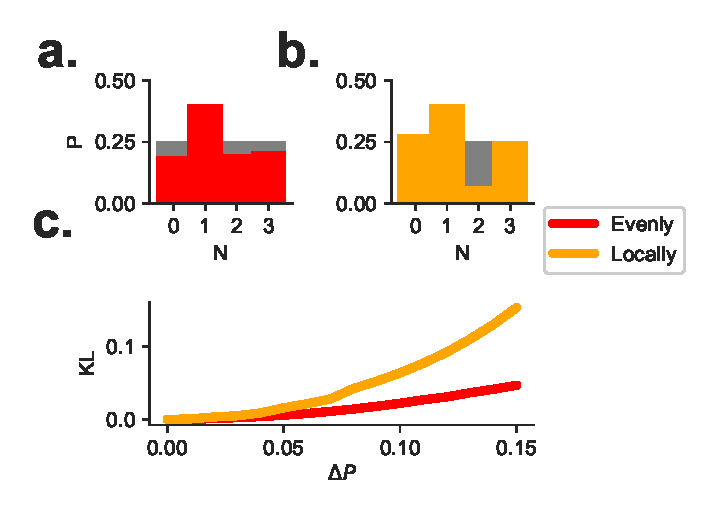
\includegraphics[width=0.4\textwidth]{figures/metrics_specifity.eps}
\caption{
\textit{Local probability structure and information value. Both distributions shown in a. and b. have the same total increase in the probability of a ``1'' appearing.
For \textbf{a.}  the necessary corresponding decrease in probabilities for all numbers (0, 2, 3) is evenly redistributed.
In \textbf{b.} the loss is focused locally on ``2''. 
\textbf{c.} The KL divergence increases more rapidly for local changes (orange) in probability density compared to an even re-distribution of probability mass (red)}}
\label{fig:metrics_specifity}
\end{figure}

\subsection*{Limitations}
A deterministic $\pi_E$ requires that the initial set of information values, $E_0$, be provided. If $E_0 = 0$, the meta-policy will never begin any exploration. While if $E_0 > 0$, theorem~\ref{theorem:opt_sub} ensures that any $E_0$, $\pi_E$ will optimal in terms of maximization of total $E$. Likewise, theorem~\ref{theorem:Z} ensures that any initial choice will not effect the optimality of the search. The magnitude of $E_0$ does not change $\pi_E$'s long term behavior, but will of course change ins transient dynamics which might be important when applying this work to real life settings. 

In our simulations we assume that at the start of learning an animal should have a uniform prior over the possible actions $A \in \mathbb{R}^K$. Thus $p(a_k) = 1/K$ for all $a_k \in A$. We transform this uniform prior into the appropriate units for our KL-based $E$ using Shannon entropy, $E_0 = \sum_K p(a_k)\ \text{log}\ p(a_k)$. 

By definition a greedy policy can't handle ties, as there is no single way to rank equal values. Our theorems~\ref{theorem:convergence} and~\ref{theorem:Z} ensure that any tie breaking strategy is valid. However like the choice of $E_0$, tie breaking can strongly effect the transient dynamics of $\pi_E$ and so can be quite important in practice. Viable tie breaking strategies taken from experimental work include, ``take the closest option'', ``repeat the last option'', or ``take the option with the highest marginal likelihood''. We do suggest the tie breaking scheme is deterministic, which maintains the determinism of the whole theory. In our simulations we use a tie breaking heuristic which keeps track of past breaks, and in a round robin fashion iterates over the action space.

Optimal exploration, both in terms of search and max $E$ does not promise that the agent has learned an accurate or unbiased memory. The loss function $\mathcal{L}_M$ is responsible for that. By comparing a memory before and after learning, information value only measures self-consistency. That is, the agent could learn a bad model of the world, but as long as it learns it consistently exploration will be consider convergent and total $E$ optimal.

Previous work studying information gain and memory has adopted an explicitly Bayesian view of animal cognition, as seen for example in \cite{Itti2009,Friston2016}. Bayesian cognition is strongly normative account, which is mechanistically and experimentally controversial \cite{TODO}. Bayesian cognition is not an assumption we require. Instead we study exploration as a simple optimization problem, whose best policy is expressed by dynamic programming.

\subsubsection*{Non-convex learning}
To simplify the problem we have assumed that the memory learning loss function $\mathcal{L}_M$ is both convex, and its gradient is always negative. Intuitively, these assumptions mean \textit{1.} there is a global solution to learning $M$ and that \textit{2.} with every observation some small amount of learning progress is made. In practice, neither assumption is realistic. Many of our most powerful learning systems are non-convex, and not all observation can and do lead to learning progress. 

There are many reasons learning can diverge. For example, a ``bad'' initialization or ``bad'' hyper-parameters, too much noise in the input data, and so on. For many complex and realistic environments, convergence of any given learning algorithm, even a convex one, is not guaranteed in the general case \cite{Mackay}. If learning does not at least begin to converge, then $E$ will not converge and $\pi_E$ must be non-optimal. This is, however, a fundamental limitation of learning theory. Still, our analysis must confine itself to agents that do learn.

If learning begins to diverge so $\triangledown \mathcal{L}_M > 0$, then $E$ must also grow (see Eq.~\ref{eq:KL}). If noise or stimulus complexity drive this momentary loss of learning progress, increases to $E$ will force the animal to ``resample'' these stimuli. The resampling order is based on the expected information gain with each. In many circumstances \textit{we conjecture maximizing $E$ will lead to $\mathcal{L}_M$ both to resume a negative trajectory and do so as efficiently or quickly as possible}. In this case, maximizing $E$ remains a sound objective. On the other hand, if $\mathcal{L}_M$ diverged due a problem with the learning algorithm itself, say a bad seed in a deep reinforcement learning model, then maximizing $E$ may exacerbate the problem leading to a potentially catastrophic feedback loop. In this case maximizing $E$ seems unsound, though it is not clear if any action policy would be better. 

\subsubsection*{Leaving local minimum}.
Local minimum are a common concrete case of that any purportedly general theory of exploration must accommodate. We've assumed $\triangledown \mathcal{L}_M < 0$. We can invert this assumption to extend our Theorems~\ref{theorem:opt_sub} and~\ref{theorem:Z} to local minimum. 

Assume instead $\triangledown \mathcal{L}_M > 0$ but this is constrained to a finite duration $W$, over an a sampling time $T$. A finite divergence like the above is half of a working definition for local minimum in $\mathcal{L}_M$. The other half being the minimum itself, defined by the gradient finding zero as $\triangledown \mathcal{L}_M = 0$.

\begin{theorem}[Local minimum] \label{theorem:local_min}
    For some learning time $T$, assuming the period $W$ for which $\triangledown \mathcal{L}_M > 0$ is finite, then the known optimal policy $\pi_E$ (per Theorem~\ref{theorem:Z} and~\ref{theorem:convergence}) is still optimal.
\end{theorem}
\begin{proof}
If for the finite period $W$, $\triangledown \mathcal{L}_M > 0$, it's logically required also that at all other times $T - W$, $\triangledown \mathcal{L}_M \leq 0$.  If $\triangledown \mathcal{L}_M = 0$ and $E_t = 0$ then there is a tie, which can be broken arbitrarily per Theorem~\ref{theorem:Z}. Now, if hold $W$ to be finite but let $T \rightarrow \infty$ then the ratio $\frac{T - W}{W}$ also must approach $\infty$. Thus by asymptotic analysis, we prove that whatever happens during $W$ will be dominated by the known optimal period, as $T \rightarrow \infty$ then $\frac{T - W}{W} \rightarrow \infty$.
\end{proof}

As we note above, there is no way in the general case to prove that any minimum is local, or that $\mathcal{L}_M$ will overcome any local minimum. We show here that if a minimum can be overcome, greedily maximizing $E$ will not interfere. We also conjecture in many cases maximizing $E$ may be the most efficient re-sampling strategy. 

% TODO: I'd like to do this proof, but am not quite sure how to form the problem statement. I don't grok KL deeply enough? Need to know more about L?

% -------------------------------------------------------------------------------------------------
\subsection*{Simulating behavior}
\textit{Note: simulations are work in progress\ldots}


\subsection*{Properties of the meta-policy} 
\subsubsection*{Sample efficiency}
The meta-policy $\pi_{\pi}$ is form a myopic control where only one of the two dual policies, $\pi^*_E$ or $\pi^*_R$, can control action selection at time. So if we define the number of state observation as the number of samples, the worst case sample efficiency for $\pi_{\pi}$ is additive in its policies. That is, if in isolation it takes $T_E$ steps to earn $E_{T} = \sum_{T_E} E$, and $T_R$ steps to earn $r_{T} = \sum_{T_R} R$, then the worst case training time for $\pi_{\pi}$ is $T_E + T_R$. There is however no reason each policy can't observe the transitions $(s_t, a_t, R, s_{t+1})$ caused by the other. If this kind of parallel learning is allowed, the worst case training time improves substantially to $\max (T_E, T_R)$. That is, learning can be done in parallel--making it cooperative--but action control is adversarial, governed by our myopic inequality $\pi_{\pi}$ (Eq.~\ref{eq:meta_greedy}).

\subsubsection*{Exploration-exploitation as an initial value problem}
In our analysis $\pi_E$ has been assumed to be deterministic. If we also restrict $\pi_R$ to be deterministic--which is sensible when optimal exploration is certain--we can the define exploration-exploitation dilemma strictly as an initial value problem, which has at least one major benefit.

Exact, turn by turn, fits are of real behavior are possible. The experimenter need only hypothesize about initial conditions. This means specifying the initial value of $E_0$ (i.e., its prior) and establishing a tie breaking rule, as well as setting the hyper-parameters. At minimum hyper-parameter tuning will require setting the learning rates for both policies in $\pi_{\pi}$ (Eq~\ref{eq:meta_greedy}), and the convergence threshold for exploration, $\epsilon$. Critically though there is no need to hand tune sampling noise \cite{Sutton2018a}.

\subsubsection*{The rates of exploration and exploitation}
In Theorem~\ref{theorem:meta} we proved that $\pi_{\pi}$ inherits the optimality of policies for both exploration $\pi_E$ and exploitation $\pi_R$ over infinite time. However this does proof does not say whether $\pi_{\pi}$ will not alter the rate of convergence of each policy. By design, it does alter the rate of each, favoring $\pi_R$. As you can see in Eq.~\ref{eq:meta_greedy}, whenever $r_t = 1$ then $\pi_R$ dominates that turn. Therefore the more likely $p(r=1)$, the more likely $\pi_R$ will have control. This doesn't of course change the eventual convergence of $\pi_E$, just delays it in direct proportion to the average rate of reward. In total, these dynamics mean that in the common case where rewards are sparse but reliable, exploration is favored and can converge more quickly. As exploration converges, so does the optimal solution to maximizing rewards.

\subsubsection*{Re-exploration}
The world often changes. Or in formal parlance, the world is non-stationary process. When the world does change, re-exploration becomes necessary. Tuning the size of $\epsilon$ in $\pi_{\pi}$ (Eq~\ref{eq:meta_greedy}) tunes the threshold for re-exploration. That is, once the $\pi^*_E$ has converged and so $\pi^*_R$ fully dominates $\pi_{\pi}$, if $\epsilon$ is small then small changes in the world will allow $pi_E$ to exert control. If instead $\epsilon$ is large, then large changes in the world are needed. That is, $\epsilon$ acts a hyper-parameter controlling how quickly rewarding behavior will dominate, and easy it is to let exploratory behavior resurface.

\subsection*{Extensions to the meta-policy}
Animals in the real world exhibit a large repertoire of behavior than simply exploration and exploitation. Without adding any new value terms, a range of other naturalistic behaviors can be mixed into our meta-policy approach. 

% TODO drop this? Leave for another paper.
% \subsubsection*{Model-free and model-based reinforcement learning}
% Reinforcement learning is divided into two general kinds, model-free and model-based \cite{Sutton2018}. % TODO explain more?
% Dual value learning offers a natural general approach to unite them. Estimating information value is a means to efficiently build a model of the world. This model can in turn be used during reinforcement learning. To that end we define two hypothetical reward policies, $\pi_F$ for the model-free rule and $\pi_M$ for the model-based.  We can then extend our original meta-policy in Eq~\ref{eq:meta_greedy} to switch between exploration, a model-free policy or the model-based policy. For example, in Eq.~\ref{eq:meta_greedy_3} we illustrate a conservative approach that switches to $\pi_M$ only once the average value of $E_t$, $\bar E$, falls below $\epsilon$.

% \begin{equation} \label{eq:meta_greedy_3}
%     \begin{split}
%         \pi_{\pi} = 
%         \begin{cases}
%             \pi_E & : E_t - \epsilon > R_t \\
%             \pi_M & : R_t \geq \bar E - \epsilon \\
%             \pi_F & : R_t \geq E_t - \epsilon \\
%         \end{cases}\\
%         \text{subject to the constraints}\\
%         R_t \in \{0, 1\}\\ 
%         p(R_t = 1) < 1\\
%         E_t - \epsilon > 0
%     \end{split}
% \end{equation}


\subsubsection*{Aversion}
Recognizing how important aversive learning was to survival in both real and artificial agents, Schmidhuber \cite{Schmidhuber1991} incorporated this is his formulation. We've meanwhile focused on reward learning in our analysis. Here we show how out myopic controller, the meta-policy, can be easily expanded to included aversive learning. When the last outcome was aversive, the animal may wish to follow a stimulus avoidance policy $\pi_A$ on the next times step. If we let $R = -1$ code for such aversive events, it is straightforward to incorporate this into a new meta-policy (Eq~\ref{eq:meta_greedy_aver}).

\begin{equation} \label{eq:meta_greedy_aver}
    \begin{split}
        \pi_{\pi} = 
        \begin{cases}
            \pi_A & : R_t < 0 \\
            \pi_E & : E_t - \epsilon > R_t \\
            \pi_R & : R_t \geq E_t - \epsilon \\
        \end{cases}\\
        \text{subject to the constraints}\\
        R_t \in \{-1, 0, 1\}\\ 
        p(R_t = 1) < 1\\
        E_t - \epsilon > 0
    \end{split}
\end{equation}


\subsubsection*{What do to by default}
If overall stimulation / motivation is too low, an animal will stop exploring or exploiting, often instead adopting some default action policy $\pi_{\emptyset}$ (e.g., grooming or checking Facebook). As a working example of this kind of meta-policy see Eq.~\ref{eq:meta_greedy_null}. Here, when the average information $\bar E$ and reward $\bar R$ fall below the exploration threshold, $\pi_{\emptyset}$ then dominates 

\begin{equation} \label{eq:meta_greedy_null}
    \begin{split}
        \pi_{\pi} = 
        \begin{cases}
            \pi_{\emptyset} & : (\bar E + \bar R) < \epsilon \\
            \pi_E & : E_t - \epsilon > R_t \\
            \pi_R & : R_t \geq E_t - \epsilon \\
        \end{cases}\\
        \text{subject to the constraints}\\
        R_t \in \{0, 1\}\\ 
        p(R_t = 1) < 1\\
        E_t - \epsilon > 0
    \end{split}
\end{equation}


% \subsubsection*{Introspection and modulation}
% TODO: for the same reason we argue reward and E are separate, we must argue E and pain are separate. A separation of cognition and affect. 
% def a pain meta policy w/ the other parts

% Pain has a stronger learning rate, so E declines quickly? Still, we think our model may be incomplete here. Suggest a adapted meta for pain and pleasure.

% Let the policies leak to tune learning rates? How much bias does this introduce. A necessary bias in a harmful world? Likewise, if you are starving tune up E for R, change epsilon. 

% Consider both ep and learning rate tuning across policies are a kind of modulation. ...If it is modulation what is its homeostasis? These must be a matched set?

% --------------------------------------------------------------------------
\section*{Discussion}
Our analysis raises the possibility that reinforcement learning on just rewards is an incomplete theory. This has been partially acknowledged by adapting information terms (as fictive rewards) into reinforcement learning problems. However we suggest that on empirical, computational, mathematical, and philosophical grounds the use fictive rewards is not far enough. Instead,  we believe information should be valued entirely for its own sake, and reward and information should be maximized separately. While this approach might seem more complex, we offer a simple optimal meta-policy for doing dual optimization. If an animal were to use this meta-policy, the classic exploration-exploitation dilemma is no longer a dilemma, and exploration can be both optimal and deterministic.

When training animals to learn a new task one of the most difficult parts in the training is constraining behavior. Left to their own devices and motivations, animals engage in a range of task-irrelevant activities. This kind of exploration is a nuisance to the experimenter, but we suggest is a important object of study for the theorist. Dual value learning accommodates the analysis and prediction for any mode of free ranging behavior, given a working definition for the state space $S$, a memory $M$, and the memory learning rule $J$.  %TODO J is right here?

% TODO: put the below somewhere?

% Having no objective of its own, exploration is generally modelled as a stochastic process. In the simple and common case of $\epsilon$-greedy, a greedy reward optimization policy is, with rate $\epsilon$, replaced by a random action, $a \sim A$ \cite{Sutton2018a}. In more complex cases, exploration has been governed by a maximum entropy approach \cite{Haarnoja2018,Haarnoja2015}. Others used visitation counts, or similar heuristics, to periodically but randomly re-visit least frequently visited past states \cite{Kulkarni2016,Sutton2018,Bellemare2016}. None of these methods though take agent learning into account, and none are guaranteed to converge. Methods that do try and converge generally rely on a variety of \textit{ad hoc} hyperparameters \cite{Sutton2018a}. 

\subsection*{Curiosity and value}.
A skeptical reader might suggest we've arbitrarily swapped an accepted term \textit{curiosity}, for another \textit{information value}. We introduce a new term for two reasons. \textit{1.} When separating information value from reward we felt it was important to place information value on principled grounds. This is why we developed the value axioms. Applying these axioms to an existing, and loosely defined term, like curiosity would seem to add confusion to the literature rather than simplify. \textit{2.}, curiosity as a subjective experience seems to dim more quickly than learning a detailed model requires. That is, learning needs more than just curiosity. We try and capture this admittedly complex motivation using information gain and the KL divergence.

\subsection*{On the axioms} 
Given that KL measures the information gain (or loss) between two models, and has a long and useful history %TODO CITE
we could have skipped the Axiomatic approach and made a direct argument for KL. We did not do this for two reasons. 

First, the value of a reward is based on its biological significance. Food, water, mates, are necessary for survival. If were are to value information for its own sake we felt it was critical to base that value not on a particular theoretical view (i.e. information theory) but instead on a firm set the theory-independent but well motivated principles. We felt obliged to first answer the question, ``If information is valuable, what do we base that value on?''. We've made one answer to that question with our axioms; We hope though ours isn't the last word.

Second, though (Shannon) information theory and KL are very useful constructs, they require symbolic and probabilistic representations. We don't know whether animals actually maintain such exact representations %\cite{TODO}. 
Likewise, in machine learning memory modules often don't rely on distributions, and instead simple recall selections of previous events (For example, \cite{Min2016}). 
Our axioms can be satisfied in these kinds of cases. Likewise, our key Theorems~\ref{theorem:opt_sub}-\ref{theorem:meta} either don't explicitly depend on information theory and KL, or can be trivially adapted to other axiomatic cases.

\subsection*{On Axiom 5} 
A skeptical reader might also find Axiom~\ref{ax:5} to be overly opinionated. A simpler natural set of Axioms is to keep 1-3 but replace~\ref{ax:5} with a new Axiom  that only requires information value track the total change in probability flux, that is $E \sim dP$. For this metric, the curves in Figure~\ref{fig:metrics_specifity} would overlap. We considered this, but felt this simpler view is incomplete. Information value should favor more specific, therefore more actionable, information. 


\subsection*{Learning structure and value}
Here we've explored only a simple probabilistic memory model that lends itself to information theoretic calculations. There are a large number of approaches an animal might use to build a model of the world. These include Bayesian structure learning, dynamical systems modeling, casual reasoning, % TODO CITE, and more.
By defining information value axiomatically, we offer a principled and consistent way to fold potentially any model-build method seamlessly and optimally into a value optimization framework. Doing this might require developing a new metric other than the KL divergence. We conjecture though that in many cases adding a simple probabilistic memory module to estimate state-action likelihoods--like the one we study here--may prove sufficient.

% \subsection*{Summary}
% Dual value learning can maximize reward and information value optimally, without letting either objective interfere or trade-off with the other. The cost is a increase in worst-case sample efficiency, when compared to the equivalent reinforcement learning problem. The severity of the cost depends on the size of the environment, and the rate of rewards.
\bibliography{library}

%%%%%%%%%% Merge with supplemental materials %%%%%%%%%%
\pagebreak
\onecolumngrid
\begin{center}
    \textbf{\large Mathmatical appendix}
\end{center}
%%%%%%%%%% Merge with supplemental materials %%%%%%%%%%
%%%%%%%%%% Prefix a "S" to all equations, figures, tables and reset the counter %%%%%%%%%%
\setcounter{equation}{0}
\setcounter{figure}{0}
\setcounter{table}{0}
\setcounter{definition}{0}
\setcounter{axiom}{0}
\setcounter{theorem}{0}
\setcounter{corollary}{0}
\setcounter{lemma}{0}
\setcounter{page}{0}

\makeatletter
\renewcommand{\suppaxiom}{S\arabic{axiom}}
\renewcommand{\suppequation}{S\arabic{equation}}
\renewcommand{\suppfigure}{S\arabic{figure}}
\renewcommand{\bibnumfmt}[1]{[S#1]}
\renewcommand{\citenumfont}[1]{S#1}

% \newtheorem{corollary}{Corollary}
% \newtheorem{axiom}{Axiom}
% \newtheorem{statement}{Statement}
% \newtheorem{theorem}{Theorem}
% \newtheorem{definition}{Definition}
% \newtheorem{lemma}[theorem]{Lemma}

\subsection*{Value axioms}
Shannon developed information theory without any sense of what information ``means''. He focused on transmitting symbols, not what those symbols refer to. This made the theory extremely general \citep{Shannon1948}. We seek a similarly general way to value information. To do this we followed Shannon's lead and developed a set axioms. But unlike Shannon we don't study how symbols in an alphabet are transmitted. We study how states from the world are remembered.

The basic idea is simple. The more memory changes when observing a state, the more valuable that observation is. It doesn't matter what that state was, only how the memory changes.

Many attempts have since been since Shannon to instill information theory with meaning and value \citep{Kolchinsky2018}. Most of these attempts require a ``salience'', or ``relevance'', or ``training'' signal (where all three terms amount to near the same thing; \cite{Deacon2015,Tishby}), while others have used evolutionary theory to create a reference \citep{Kolchinsky2018,Deacon2015}. Here we require no outside reference to estimate value. 

To state the axioms first we need to introduce some notation and definitions. We ask for a bit of patience from the reader. The definitions are necessarily abstract, as we are developing a theory of information value that is independent of any particular model of animal cognition or learning.

\subsubsection*{States and actions}
Here we study a number of $N$ finite states $s$ in a world $s \in S^N$. This is analogous to Shannon's initial formulation of symbols $x$ in an alphabet $X$. A state might be a visual scene \cite{Mnih2015}, or an odor vector \cite{Dasgupta2017,Calhoun2014}, an index into a symbol table, or a set of spatial coordinates, or any set of numbers, vectors, or tensors. All that matters is the states are unique and self-consistent in $S$ and that they do not change with time or with experience. 

We limit the number of actions $a$ animal might take to a finite set $A$ of size $K$, $a \in A^K$, Like $S$, we allow the set $A$ to conceivably be any set of numbers, vectors, or tensors.

\subsubsection*{A definition of memory}
A memory $M$ is a set of transformed states, defined recursively by the encoder $f$ as $M \leftarrow f(M, s)$. The base case for $M$ is said to be the empty set $M_{0} = \emptyset$. In defining $f$ we assume the encoding  of any $s$ can, in principle, create or modify multiple memories in $M$. That is we do not assume a bijection  and not only one element $m_i \leftarrow f(s, m_i)$ from $M = \{m_1, m_2, m_i, \ldots\}$. We do not require $M$ be finite like $S$ which means in theory it's possible to form more memories than there are states. 

We require that the memory $M$ can decoded by function $g$ to produce recollection $z$ by $g(M, s) \rightarrow z$. We don't concern ourselves with details of $z$. They are as open as the definition of states in $S$.

We define time $t$ as a index of sequential state observations of $s \in S$, such that $t = (0,1,2,3,\ldots,T)$.

To finish our definition of $M$ we add one critical restriction to the encoder $f$: it must be invertible. That is, if there exists $M_{t+1} = f(M_{t}, s)$ then there must also exist an inversion $f^{-1}$ so $M_{t} = f^{-1}(M_{t+1}, s)$. 

We summarize the requirements for memory $M$ in Definition~\ref{def:memory}.

\begin{definition}
\label{def:memory}
We define a memory $M$ as a potentially infinite set, defined over a finite state space $s \in S^N$, whose elements are added by an invertible encoder $f$ such that $M_{t+1} = f(M_{t}, s)$ and $M_{t} = f^{-1}(M_{t+1}, s)$. Elements $z$ from $M$ are recovered by a decoder $g$, such that $z = g(M, s)$. The initial memory $M_{0}$ is the empty set, $M_{0} = \emptyset$.
\end{definition}

Definition~\ref{def:memory} covers simple and complex ideas of a memory. In the simplest case where $f$ and $g$ are identity functions, then $M$ is just a simple direct record, or subset, of the states observed by the animal $M \subseteq S$. If $f$ is a probability function, $0 \geq f(s) \leq 1; \sum_{S}^{i} f(s_i) = 1$, then $M$ is a distribution over $S$, and $g(M, s_i) = p(s_i)$. Likewise, if $f$ is not only a probability function implements Bayes' rule, then $M$ can be a conditional distribution. In principle Definition~\ref{def:memory} also encompass hierarchical Bayesian learning, VAE and other generational approaches found in modern machine learning / artificial neural networks, as well as sequential and recurrent memories, like echo state networks, FORCE, LTSM and GRU. It also extends also to cases not often considered memories \textit{per se} but which include an encoder-decoder pair-- including dimensionality reduction techniques (\textit{e.g.} PCA, NMF, tSNE), clustering methods (KNN), and mixture models (GMM, kernel).

Several of these methods--especially those we've labeled as more complex--are defined implicitly or explicitly with an encoder and decoder. Most do not explicitly or implicitly include a inverse decoder $f^{-1}$. However all we require is that $f^{-1}$ could be constructed, \textit{in principle} (Theorem~\ref{theorem:opt_sub}).

\subsubsection*{Memory space}
As we'll seen in the next section, to make information value axiomatic we rely on comparing sequential changes to the memory $M$, as it moves from $M_{t}$ to $M_{t+1}$. This comparison is made using a distance metric $d(x,y)$, which is minimally constrained by $d(x,y) \geq 0$ and $d(x,y) = 0$ if and only if $x = y$. We do not require that $d$ obeys the triangle inequality, nor that is be symmetric. 

% TODO: is this precise enough? Do I need to say what x and y are?
\begin{definition}
\label{def:distance}
We define a distance $d$ to be any function where $d(x,y) \geq 0$ and $d(x,y) = 0$ if and only if $x = y$.
\end{definition}

The distances for two sequential memories $M_{t}$ to $M_{t+1}$ are measured using the distance $d$ on the decoded set of memories $d(z_{t+1},z_{t})$. This assumption let's us separate the definition (and eventual implementation) of $M$ from the distance $d$.

\subsubsection*{The value axioms}
We denote information value as $E$, subject to the following axiomatic constraints. Under each formal Axiom, we offer an informal summary.

\begin{axiom} 
    $E$ is a function which measures the distance $d$ between $M_{t+1}$ and $M_{t}$ to a real number, $E: (M_{t+1}, M_{t1}) \rightarrow \mathbb{R}$.
    \label{ax:1}
\end{axiom} \\
\noindent
Value is subjective, and so should only depend on an animals memory. (Working with just sequential memories,$M_{t+1}$ and $M_{t}$ and scalars, simplifies the problem mathematically.)

\begin{axiom}
    $E \geq 0$.
    \label{ax:2}
\end{axiom}
\noindent
New information about the world is always valuable, even if its later consequences might not be. The consequences of the information may not always be good, but that's a separate issue.

\begin{axiom}
    $E = 0$ if and only if $M_{t+1} = M_{t}$.
    \label{ax:3}
\end{axiom}
\noindent
If you remember something perfectly, there is no value in learning it again.
 
\begin{axiom}
    $E$ is strictly monotonic with the total change in $d$ measured between $M_{t+1}$ and $M_{t}$.
    \label{ax:4}
\end{axiom}
\noindent
The information value should track the total change in memory. 

\begin{axiom}
    $E$ is monotonic with the compactness $C$ (Eq.~\ref{eq:compactcude}) of $d$ measured between $M_{t+1}$ and $M_{t}$.
    \label{ax:5}
\end{axiom}
\noindent
Specific information is more always more valuable than less specific information. (We use geometrical compactness as surrogate for specificity, which doesn't seem to have a precise meaning.)
\\ \\
The compactness $C$ of a hyper-cube has a simple formula, $C = \frac{P^2}{A}$ where $P$ is the cube's perimeter and $A$ is its area. Therefore as $M_{t}$ moves to $M_{t+1}$, the we can measure the distances $\{d_i, d_{i+1}, d_{i+2},\ldots d_{N}\}$ for all $O \leq N$ observed states $Z$, such that $Z \subseteq S$ and treat them as if they formed a $O$-dimensional hyper-cube. In measuring this imagined cube we arrive at a geometric estimate for change the compactness of our memory $M$ (Eq.~\ref{eq:compactcude}).

\begin{equation} \label{eq:compactcude}
\begin{split}
    C & = \frac{\Big ( 2 \sum_{O}^{i} d_i \Big )^2}{\prod_{O}^{i} d_i}
\end{split}
\end{equation}

% Our Axiomatic and self-referential approach to information value is extremely general for the same reasons as Shannon's original theory: we examine how memory changes with learning, but do not consider what the memory refer to in the world; what it means. Memories are just a collection of (transformed) states (Definition~\ref{def:memory}). 


\subsection*{Information value as a dynamic programming problem}
To use theorems from dynamic programming we must first prove our memory $M$ (Definition~\ref{def:memory}) has a special property--``optimal substructure''. Optimal substructure means one can take a series of observations, and break into to a smaller number of sub-problems or series. If these series/sub-problems have \textit{optimal substructure} they will inherit the relevant optimality present in the original series. That is, if the full series is optimal in some sense all its sub-problems are optimal too. The question for any series is then, ``What are the sub-problems that inherit optimality''. By proving we can decompose $M$ optimally--that it has optimal substructure--we also prove that we can grow the series optimally; induction proofs become trivial when the optimal substructure is known. 

We prove the optimal substructure of $M$ of a sequence of state observations. To make these observation we must introduce additional notation. We've previously introduced time $t$ as an index of observed states, but introduced no mechanism for making state observations. 

We formalize the state observation process with two functions, an action policy function $\pi$ and a transition function $\delta$. In informal terms the transition function is an abstract stand in for the world or environment in which animal lives, and the policy represents it's total capacity for value-based decision making.

\begin{definition}
    \label{def:policy}
    Let $\pi$ be a policy function that maps a state $s$ to an action $a$, $\pi : s \rightarrow a$, such that $s \in S, a \in A$.
\end{definition}

\begin{definition}
    \label{def:transition}
    Let $\delta$ be a transition function which maps $(s_{t},a_t)$ to a new state $s_{t+1}$, $\delta : (s_{t}, a_t) \rightarrow s_{t+1}$.     
\end{definition}

By combining policy function $\pi$ with transition function $\delta$, we can generate a sequence of observations, adding these to the memory $M$. Given some initial state $s_{t}$, apply $\pi$ to produce an action $a_t$, $a_t = \pi(s_{t})$. Given $a_t$ and $s_{t}$ we can apply the transition function, to produce the next observation, $s_{t+1} = \delta (s_{t},a_t)$. This cycle then repeats, generating a sequence of observations indexed, as we've stated, by $t$.

% A policy function and transition function combine to generate a path $P$. We use $t$ to index into $P$. 

% \begin{definition}
%     Let $P$ be a finite ordered collections of states $s$, such that $s \in S$ and the length of $P$ is $T$. We define $P$ recursively, $P(t+1) \leftarrow \Lambda(P(t), \pi(P(t)))$ for some policy $\pi$.
% \end{definition}

For consistency with standard notation for dynamic programming and the Bellman equation (which comes into play below) we redefine $E$ in terms of a classic payoff function, $F(M_{t}, a_t)$. We defined $E$ axiomatically based exclusively on $M$ and $d$. We will use Definitions~\ref{def:policy} and~\ref{def:transition} to redefine $E$ in terms the current memory $M_{t}$ and the next action, as set by $\pi$. This brings us to Definition~\ref{def:payoff}. The axiomatic form of $E(M_{t+1},M_{t}$ and the payoff form $F(M_t, a)$ are interchangeable. We switch between there notation as needed.

\begin{definition}
    \label{def:payoff}
    Let $F(M, a)$ be payout function for $E$ as defined by Eq.~\ref{eq:payout}.
\end{definition}

\begin{equation}
    \begin{split} \label{eq:payout}
    F(M_{t}, a_t) = E(M_{t+1}, M_{t})\\
    \text{subject to the constraints} \\
    a_{t} = \pi(s_t) \\
    s_{t+1} = \delta(s_{t}, a_t),\\ 
    M_{t+1} = f(M_{t}, s_{t})
    \end{split} 
\end{equation}

Using Eq~\ref{eq:payout} we can write down the total information value, as the sum of all payout functions for some policy $\pi_E$ made over some observation period $T$, where $t = (1,2,3,\ldots,T)$. This is value term our dynamic programming solution will maximize.

\begin{equation} \label{eq:V}
    \begin{split}
        V_{\pi_E} = \sum_{t \in T} F(M_{t}, a_t)\\
    \end{split}
\end{equation}

% --------------------------------------------------------------------------
\subsubsection*{A proof of optimal substructure}
A first step in solving a dynamic programming problem is isolating the relevant sub-problem, and proving it has an optimal substructure -- that the problem can be decomposed into an iteratively optimal series. 

\begin{theorem}[Optimal substructure] \label{theorem:opt_sub}
    Assuming transition function $\delta$ is deterministic, if $V^*_{\pi_E}$ is the optimal information value given by $\pi_E$, a memory $M_{t+1}$ has optimal substructure if the the last observation $s_t$ can be removed from $M_t$, by $M_{t+1} = f^{-1}(M_{t+1}, s_t$ where the resulting value $V^*_{t-1} = V^*_{t} - F(M_t, a_t)$ is also optimal. 
\end{theorem}
\begin{proof}
    Given a known optimal value $V^*$ given by $\pi_E$ we assume for the sake of contradiction there also exists an alternative policy $\hat \pi_E \neq \pi_E$ that gives a memory $\hat M_{t-1} \neq M_{t-1}$ and for which $\hat V^*_{t-1} > V^*_{t-1}$. 

    To recover the known optimal memory $M_t$ we lift $\hat M_{t-1}$ to $M_t = f(\hat M_{t-1}, s_t)$. This implies $\hat V^* > V^*$ which in turn contradicts the purported original optimality of $V^*$ and therefore $\hat \pi_E$.
\end{proof}


\section*{Information value and search}
\subsection*{An assumption of learning progress}
The study of information geometry models learning as an approach to information equilibrium. As learning progress plateaus, variance decreases, and therefore so does entropy. The rate at which learning plateaus is governed by the Fisher information metric, which is the hessian of the KL-divergence.

% HERE: re-watch Baez talk...

Exploration depends on learning progress. We assume that every every state observation is accompanied by change in $M$. This change can be arbitrarily small, but must be non-zero. 
% To make our proofs work we assume each observation $s$ is learned--to some small degree perhaps--by the memory $M$. Formally then, and with \textit{a loss of generality}, we assume that $\mathcal{L}_M$ is convex, and that every observation $s$ leads to learning progress on the memory $M$. Unless, that is, $\mathcal{L}_M(s) = 0$. That is, the gradient of $\triangledown \mathcal{L}_M < 0$ for all $s \in P$ when $L(s) \neq 0$. If $\triangledown \mathcal{L}_M = 0$, then for a convex learner we are at the global minimum, and so exploration and learning should cease. Having completed our initial proofs we then show under what conditions these assumptions can be relaxed.

\subsection*{Sorting preliminaries}
Our proofs for exploration are really sorting problems. If every state must be visited (or revisited) until learned, then under a greedy policy every state's valie must--at one time or another--be the maximum value. 

Sorting requires ranking. Ranking requires that we make a definition for both the greater $>$ and less than inequalities $<$. For three real numbers, ${a,b,c} \in \mathbb{R}$.

\begin{definition} \label{def:ineq}
    \begin{align}
        a \leq b \Leftrightarrow \exists c; b = a + c \\
        a > b \leftrightarrow (a \neq b) \wedge (b \leq a) 
    \end{align}
\end{definition}

\subsubsection*{A greedy information policy will explote completely}
% TODO need intro.....

% we let $ F_0 = 0$, talk about f_0 > 0. Somew

\begin{definition}
    Let $Z$ be set of all visited states, where $Z_0$ is the empty set $\{\}$ and $Z$ is built iteratively over a path $P$, such that $Z = \{s | s \in P\ \text{and}\ s \not\in Z\}$.    
\end{definition}

\begin{theorem}[State search -- completeness and uniqueness] \label{theorem:Z}
A greedy policy $\pi$ is the only deterministic policy which ensures all states in $S$ are visited, such that $Z = S$.
\end{theorem}
\begin{proof}    
    Let $\mathbf{E} = (E_1, E_2, ...)$ be ranked series of $E$ values for all states $S$, such that $(E_1 \geq E_2, \geq ...)$. To swap any pair of values ($E_i \geq E_j$) so ($E_i \leq E_j$) by Def.~\ref{def:ineq} $E_i - c = E_j$.  

    Therefore, again by Def.~\ref{def:ineq}, $\exists \int \delta E(s) \rightarrow -c$. 

    \textit{Recall}: $\triangledown \mathcal{L}_M < 0$

    However if we wished to instead swap ($E_i \leq E_j$) so ($E_i \geq E_j$) by definition $\not \exists c; E_i + c = E_j$, as $\not \exists \int \delta \rightarrow c$. 

    To complete the proof, assume that some policy $\hat \pi_E \neq \pi^*_E$. By definition policy $\hat \pi_E$ can any action but the maximum leaving $k-1$ options. Eventually as $t \rightarrow T$ the only possible swap is between the max option and the $kth$ but as we have already proven this is impossible as long as $\triangledown \mathcal{L}_M < 0$. Therefore, the policy $\hat \pi_E$ will leave at least 1 option unexplored and $S \neq Z$.
\end{proof}

\begin{theorem}[State search -- convergence] \label{theorem:convergence}
    Assuming a deterministic transition function $\Lambda$, a greedy policy $\pi_E$ will resample $S$ to convergence as $t \rightarrow T$, $E_t \rightarrow 0$.
\end{theorem}
\begin{proof}
    \textit{Recall}: $\triangledown \mathcal{L}_M < 0$. 

    Each time $\pi^*_E$ visits a state $s$, so $M \rightarrow M'$, $F(M', a_{t+1}) < F(M, a_t)$

    In Theorem~\ref{theorem:Z} we proved only deterministic greedy policy will visit each state in $S$ over $T$ trials.
    
    By induction, if $\pi^*E$ will visit all $s \in S$ in $T$ trials, it will revisit them in $2T$, therefore as $T \rightarrow \infty$, $E \rightarrow 0$. 
\end{proof}

If the transition function $\Lambda$ is stochastic, the noisy state changes will prevent $E$ from fully converging to 0. This might be ideal, as it will force continual re-exploration of the world. However if we redefine the converge of $E$ not to 0 but to some criterion $\epsilon$, we can once again ensure convergence in noisy worlds. That is, in the limit of $t \rightarrow T$, $E_t \rightarrow \epsilon$, where $0 leq \epsilon \ll E_0$ with $E_0$ denoting the initial value of $E$. Too large though, and $\epsilon$ will interfere with potential optimality of $\pi^*_E$ (by Theorem.~\ref{theorem:Z}). 


\twocolumngrid
\end{document}
